%
% File: chap02.tex
% Author: ta16969
% Description: !!!!!!!!!.
%
\let\textcircled=\pgftextcircled
\chapter{Artemis Design and Implementation}
\label{Artemis Design and Implementation}

\initial{T}his chapter introduces and explains the implementation of Artemis; Introducing key features identifying \texxit{how} Artemis was developed and the the overarching design values used to focus development i.e. OER, Captology (Web Credibility), Security and Accessibility.


\section{Development Tools and Languages}

Artemis has been developed using the XAMPP-VM so as to use XAMP for Linux within the OS X environment, using the convienience of the OS X hypervisor to emulate a development environment that can be expected of industry standard production \cite{ApacheFriends.org}. Therefore Artemis has been predominantly written in PHP, is served by Apache and uses MariaDB (an SQL Database). An alternative  JS and NoSQL full stack was considered, specifically the MeteorJS full stack; however it stands to reason that MeteorJS is too niche and unsuitable for the OER modality of the tool and desired longevity in the Open Source community. Furthermore a conventional SQL oriented stack is considered desirable for building a social network as evidenced by the experience of the lead developers of Disapora an Open Source social network that had to infamously migrate from MongoDB to SQL \cite{Mei}.

Cross browser compatibility is outside of the scope of this project. However during development and evaluation the product has been used indiscriminately between Google Chrome, Mozilla Firefox (Developer Edition) and Safari. This approach helped target niche vendor specific issues, however it is stressed that complete cross compatibility is beyond the scope of the project and has not been explicitly attempted beyond the general good development practice of using multiple industry leading browsers.







\section{Stakeholder Assessment and Participation}

In an earier sub-section titled  \textit{Three Principle Stakeholders} it was determined that to enable a desirable pedagogy it would be prudent to investigate the primary stakeholders of a flexible pedagogy \cite{Gordon2014}; i.e. the UoB TEL team, CS course instructors and the student cohort are to be considered so as to ensure the successful development, deployment and adoption of the solution. Therefore the values of the Primary Stakeholders was sought and incorporated into Artemis as follows, within the reasonable constraints of the project (The following is an overview of the work done and specific references towards the work done will be made when relevant):

\begin{itemize}
    \item \textbf{TEL Team}: The TELED (Technology Enhanced Learning and Education Development)  department at the University of Bristol has a wide mandate that mandate that broadly seems to straddle procurement, deployment, adoption, training and research associated with TEL solutions at the UoB \cite{UniversityofBristol}. An informal meeting was sought with the TEL team, which resulted in a valuable opportunity to personally discuss the project with the entire team who have a first hand experience of past, present and future TEL projects deployed at the UoB and their development criteria, as well as experience in identifying what leads to failed as opposed to successful adoption within the context of TEL solutions deployed at the UoB. It is interesting to note that the TEL team cited lack of instructor adoption, as opposed to student's adopting a technology as equally important to the latter. Indeed the meeting also revealed a declining interest in the use of student forums, which may make a social network a desirable outcome of this project (as the former is viewed as a dated solution).
    
    \item \textbf{Teachers}: Feedback from UoB course instructors was sought via informal interviews; Primarily from Dr David Bernhard and Dr Ian Holyer. The TELED department had specifically indicated that there was a lack of instructor interest/adoption in TEL solutions specifically at the CS department and this was elaborated upon by the CS instructors interviewed. It was primarily cited that most TEL solutions were not adopted for either or both of the following reasons:
    
    \begin{itemize}
        \item Poor or unreliable functionality.
        \item Poor or faulty visual aesthetics.
    \end{itemize}
    
    
    The rationale for lack of adoption cited can be corroborated against the values of \textit{Web Credibility} and persuasive design, which are discussed in greater detail in a later section but indicate that users are less like to adopt a technology if it is faulty or it does not seem to be professionally designed. The findings of the aforementioned are embedded in the GUI design and also used as the basis of evaluating Artemis and subsequently refactoring it's source code; Addressing the aforementioned instructor values. Furthermore iterative feedback was sought from them during the development of the project for their opinions and advice regarding the aesthetic layout of the interface and desired functionality.


    \item \textbf{Students}: Possibly the most important of the three stakeholders as the majority of the users are expected to be students. UoB CS conversion students and CS undergraduate student values were incorporated into Artemis via the following exercises:
    
    \begin{itemize}
        
        \item \textbf{Focus Group}: An arbitrary group of people from the MSc and BSc Computer Science cohort were asked to participate in a brain storming session to help generate creative ideas for the proposed social  network. The underlying purpose was to generate creative ideas,use cases and possible modalities. The overarching outcome of this exercises was that there was a desire for a Facebook-StackoverFlow styled hybrid social network, as opposed to other mainstream social networks such as Twitter or Reddit(As corroborated by the TELED department,most students expressed a distaste for the relatively \textit{old fashioned} forums currently used at the UoB, which have an interface similar in substance to Reddit).

        \item \textbf{Open Ended Evaluation and Refactoring}:  A group of ten people from the MSc and BSc Computer Science cohort were asked to participate in an Open Ended Evaluation (Appendix A1). The purpose of this evaluation was to assess and improve the Web Credibility of the Artemis UI and UX  and find any bugs or anomalies in the code. The results were subsequently used to refactor the source code and improve the UI (thus enhancing the underlying rationale of making it a \textit{Persuasive Technology} as discussed under the section in the chapter titled \textit{Persuasive Web Design}).
        
        As part of the  evaluation participants were asked to perform a series of use cases. The purpose of this step was to encourage the rigorous evaluation of all feature of Artemis. However users were also strongly encouraged to explore Artemis and try to maliciously break or damage the program (so as to cover use cases that might not have been envisioned). Furthermore users were required to test the application \textbf{unassisted} and without intervention, as is reasonably possible.
        
        The approach yielded thorough feedback and bugs in Artemis. Therefore the code was subsequently refactored and improvements to the User Interface were made. These have been identified and discussed in the chapter on evaluation.
        
        
    \end{itemize}
    
\end{itemize}

 
\section{Persuasive Web Design}

At the core of a rationale for embedding  learning models \& methodologies, pedagogy and social networks to ultimately develop a TEL solution is the presumption that the application will influence it's users. A TEL solution unable to persuade users in a desirable manner, due to either lack of adoption or otherwise inefficacy, is a solution that will fail or perform poorly; A fact outlined via preliminary informal discussions with the TEL team at the UoB.

The broad research area of \textit{captology}, by the Stanford Persuasive Technology Lab (STPL) covers the somewhat controversial study of  how computer and applications can be designed to change what people think and do \cite{Fogg2002a,Fogg2002,Fogg2001,Fogg1999}. Whilst extensive research of this area is deemed beyond the constraints of the project, some consideration is given to the constituent factors that improve user acceptance and/or influence; \textit{Web Credibility} and resultantly \textit{Web Application Security} and \textit{User Accessibility}.

It is proposed that by enhancing web credibility and application security, security the TEL solution can be designed in a manner that enhances user acceptance and adoption; Effectively not just making the TEL solution more effective in achieving it's intended purpose, but also avoiding a common  underlying cause of failure for TEL solutions implemented at the UoB i.e. lack of adoption of applications by relevant users due to poor reliability,aesthetics, accessibility and usability. Indeed the underlying cause of failure was corroborated by instructors in the CS department who did not use certain TEL solutions available to them due to broken functionality or poor aesthetics i.e. Core issues against which the STPL advises so as to increase an application's \textit{Credibility} \cite{Fogg2002a,Fogg2002,Fogg2001,Fogg1999} and enhance application adoption or usage.








\subsection{Web Credibility}

One aspect of making a \textit{persuasive} TEL solution, is by enhancing \textit{web credibility}. Web credibility within the context of designing this TEL solution refers to embedding best practice within web design, so as to influence a user's perspective of trustworthiness of the tool itself \cite{Fogg2001,Fogg2002} i.e. making the social network ultimately more persuasive and fit for purpose, by improving user perceptions of reliability and trustworthiness of the application \cite{Fogg2001} and effectively improving user acceptance.


In view of the project constraints, it is proposed that web credibility for the proposed web application can be achieved by adopting  the \textit{Stanford Guidelines for Web Credibility} \cite{Fogg2002a}. These guidelines are effectively a condensed and easy to follow framework for developing a Web Credible application based on the extensive research carried out by the STPL and associates; effectively aiding web developers to enhance web credibility based on the findings of quantitative research as opposed to mere intuition \cite{Fogg2002a,Fogg2002,Fogg1999}.

These are listed as follows and briefly explained within the context of developing Artemis  and it's use cases:

\begin{enumerate}
    \item \textbf{"Make it easy to verify the accuracy of the information on your site ?"} \cite{Fogg2002a}:
    
    The recommendation by STPL here is to allow for third party assurances such as citations, references and source material \cite{Fogg2002a}. There are several ways that this can be embedded in the design of a proposed social network. This was implemented and embedded in Artemis as follows:
    \begin{enumerate}
        
        \item As illustrated in a previous use case in \textbf{Figure \ref{fig:UseCaseParticipatory}}, a participatory learning model has been adapted to illustrate the underlying rationale for selecting a social network as an appropriate  modality for the TEL solution. It is envisaged that instructor intervention and scrutiny from the rest of the cohort will make it easy to verify the authenticity of the information. An illustration of a possible case where this can happen is illustrated below:
            
        \begin{figure}[H]
        	\centering
        	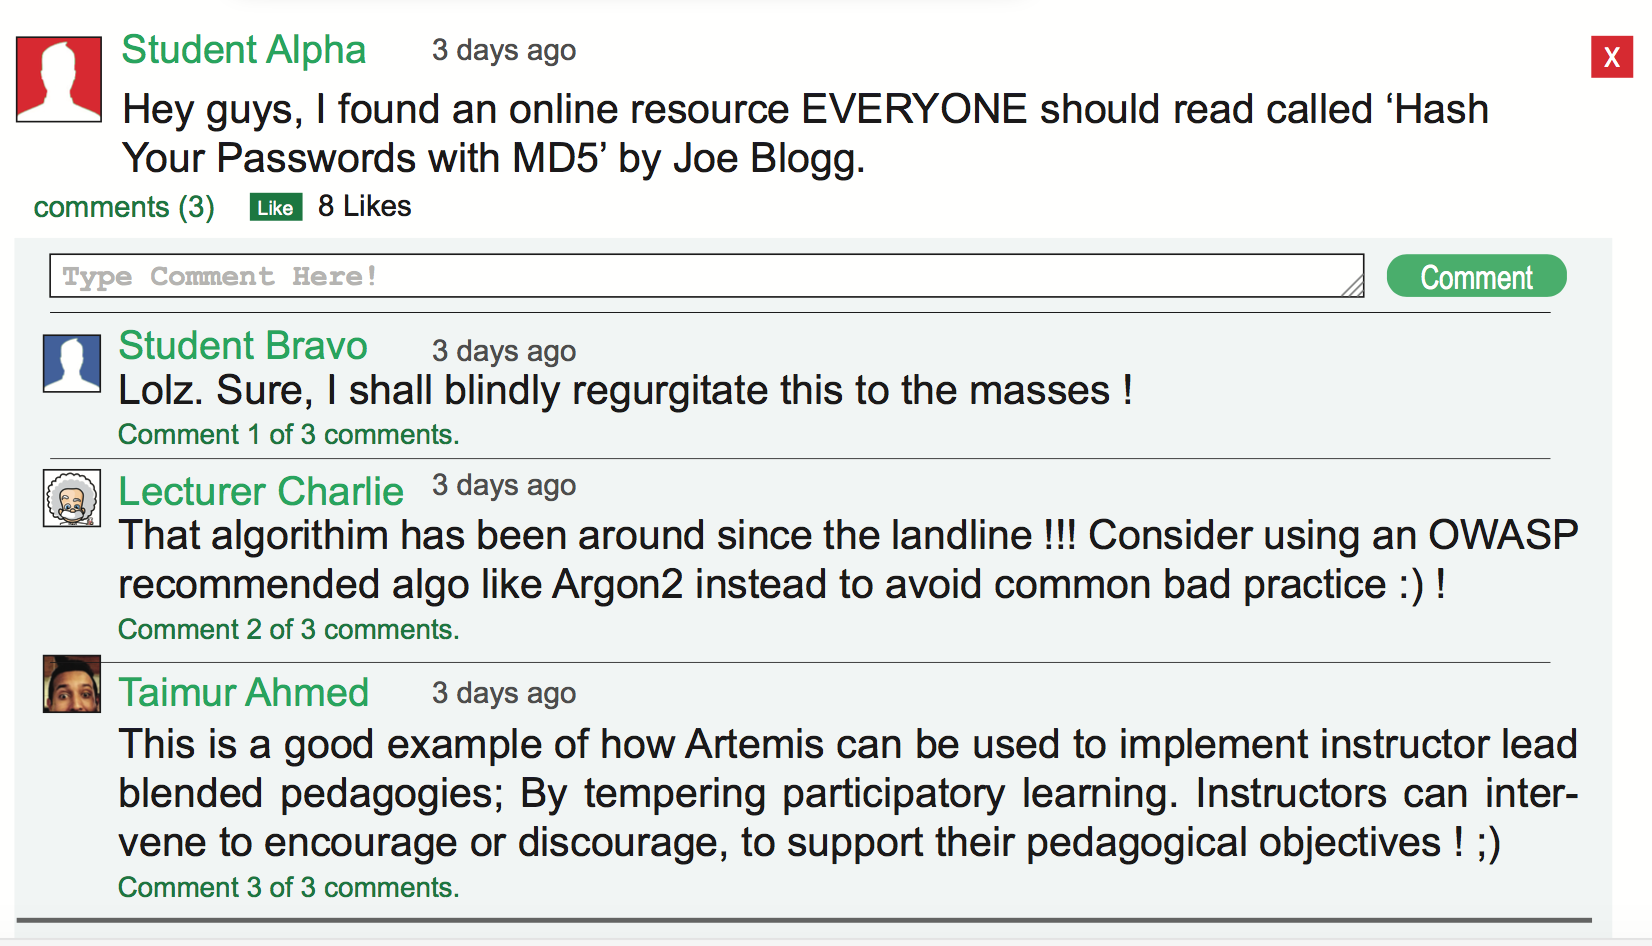
\includegraphics[scale=0.45,right]{chapters/chapter03/figures/comment.png}
        	\mycaption[Illustration of  Use Case, depicting possible adaptation of Participatory Learning Model to Proposed Social Network]{Illustration of  Use Case, depicting possible adaptation of Participatory Learning Model to Proposed Social Network}
        	\label{fig:UseCaseParticipatory}
        \end{figure}
        
        This possible use case (illustrated in previous figure) was also proposed during the focus group as well and the likelihood of it instructor intervention corroborated via course instructors. It was agreed upon by consensus that it is a reasonable assertion that when material is shared on Artemis it can easily be verified by other students, course instructors or teaching assistants via post \textit{likes} and \textit{comments}.
    
    \end{enumerate}
    
    \newpage
    \item \textbf{"Show that there's a real organization behind your site"} \cite{Fogg2002a}:
    
    A significant amount of development effort has been put into creating documentation for Artemis. Whilst the documentation has a wide and varied scope or purpose, it is essential to note that it indicates towards the existence of a professional team behind the project. A list of the documentation made readily accessible to Artemis users (i.e. always available in the application) is as follows:
    
    \begin{itemize}
    
        \item A \textbf{Wiki page} for Artemis so that users can find details about the project, underlying rationale, the programme specifications, legal modalities and information about the developers.
            \begin{figure}[H]
                \centering{ 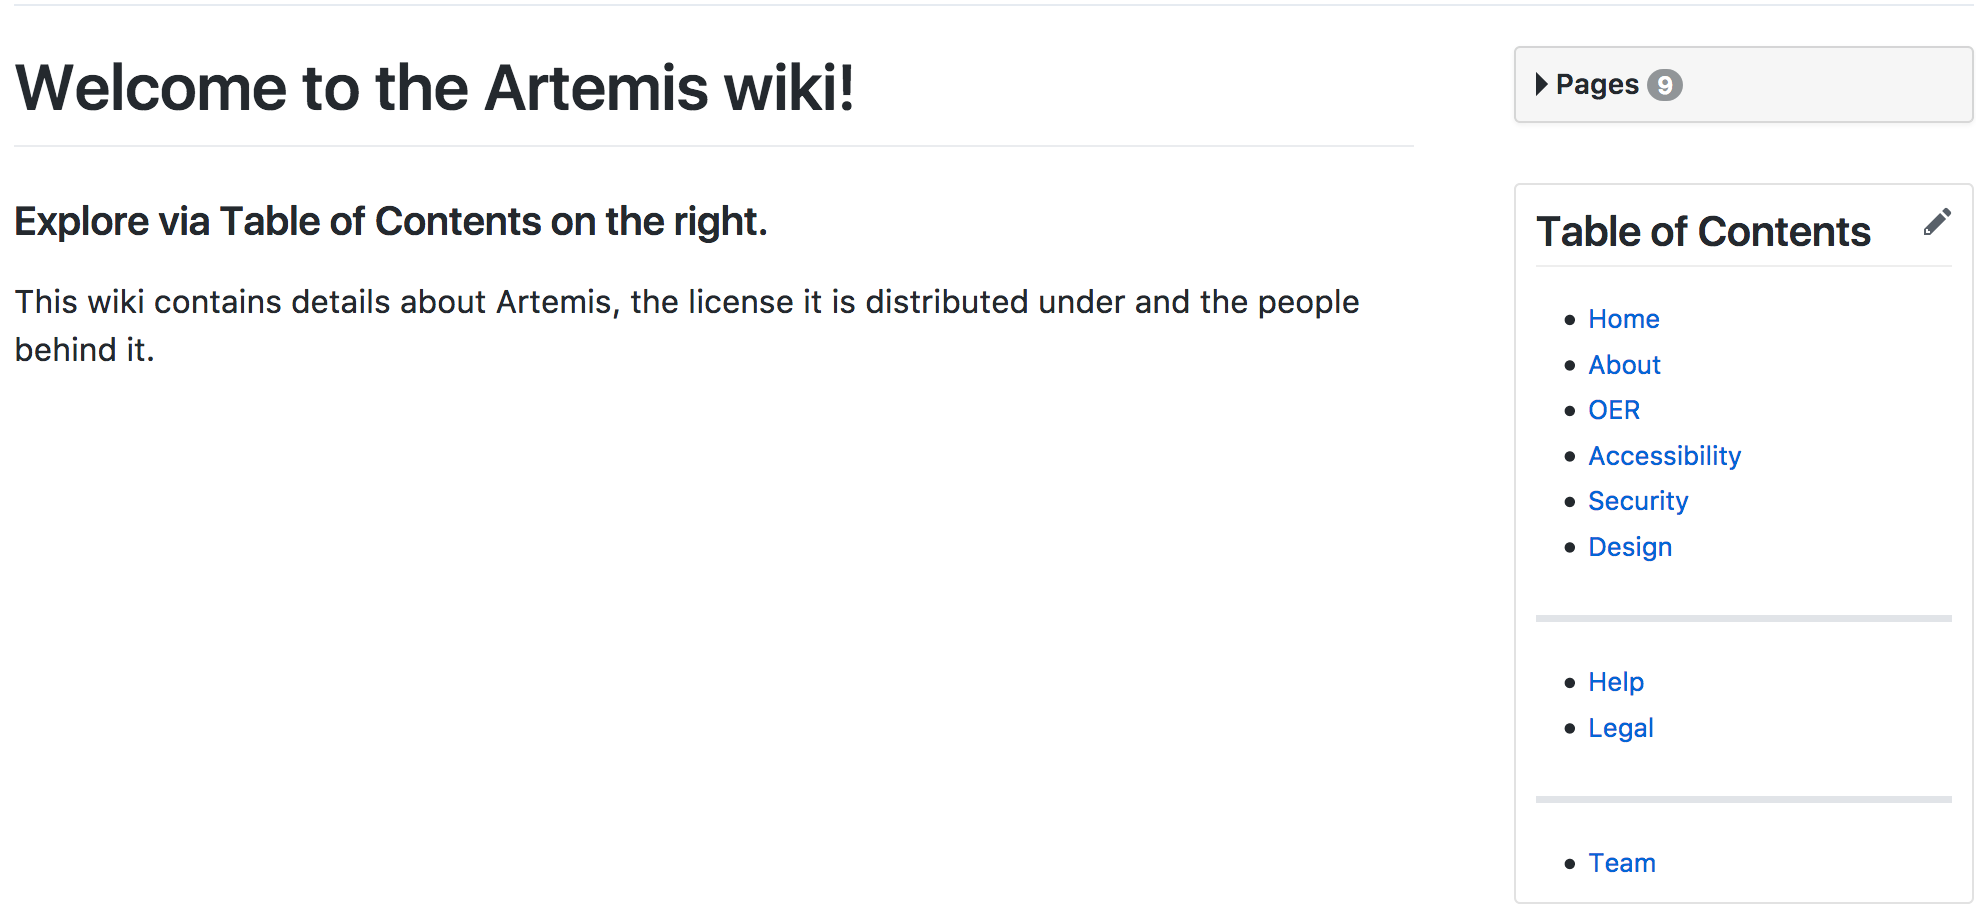
\includegraphics[scale=0.36]{chapters/chapter03/figures/Wiki.png}}
                \label{wiki}
                \caption{Artemis Wiki page. Available at: \url{https://github.com/TaimurAhmed/summerProject2017/wiki}}
            \end{figure}
            
        \item A \textbf{User Feedback and Bug Reporting page} on GitHub to so that users may report bugs and track issues. It also provides developers with a forum to discuss details of bugs, give feedback and reports as depicted in the following figure.
            \begin{figure}[H]
                \centering{ 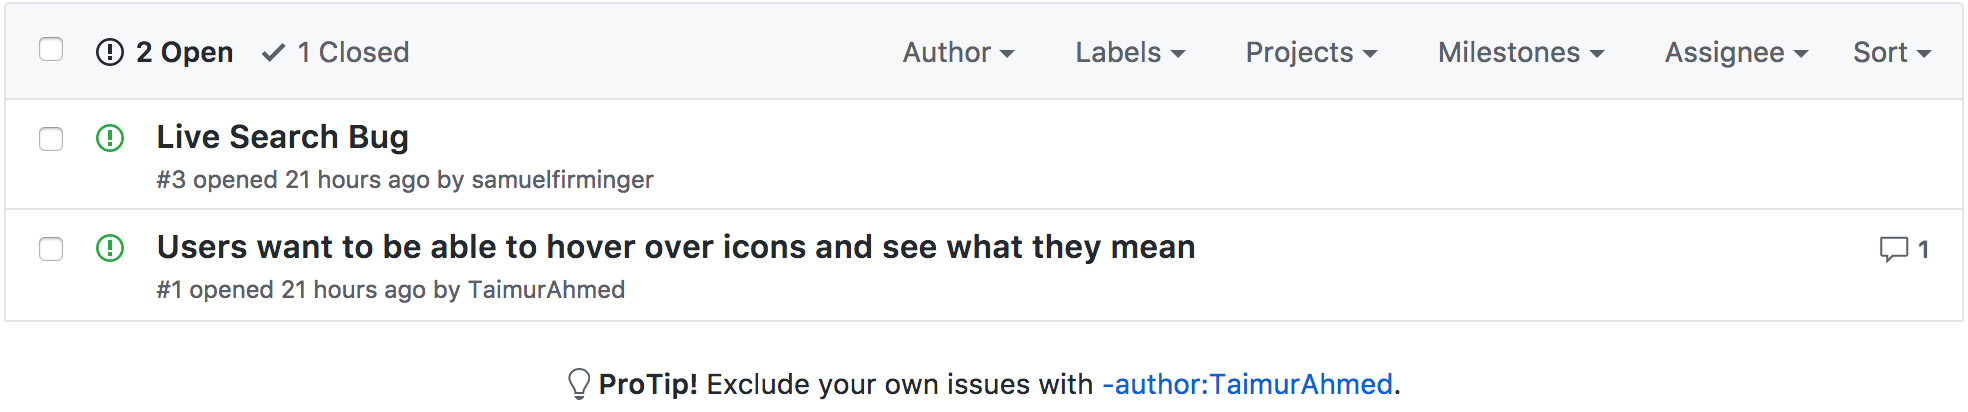
\includegraphics[scale=0.36]{chapters/chapter03/figures/bug.png}}
                \caption{Artemis Bug Report and Issue Tracking Page. Available at: \url{https://github.com/TaimurAhmed/summerProject2017/issues}}
            \end{figure}
        
        \newpage
        
        \item A \textbf{Developer Profile page} has been linked to the Wiki and can be accessed through the navbar.
            \begin{figure}[H]
                \centering{ 
\includegraphics[scale=0.36]{chapters/chapter03/figures/profile.png}}
                \label{developer}
                \caption{Developer Profile Page with contact details. Available at: \url{https://github.com/TaimurAhmed}}
            \end{figure}
        
        \item A \textbf{ReadMe markdown file} on GitHub for other developers. This is standard practice in most Open Source projects that want other developers to be able to understand and work on the project.
            \begin{figure}[H]
                \centering{ 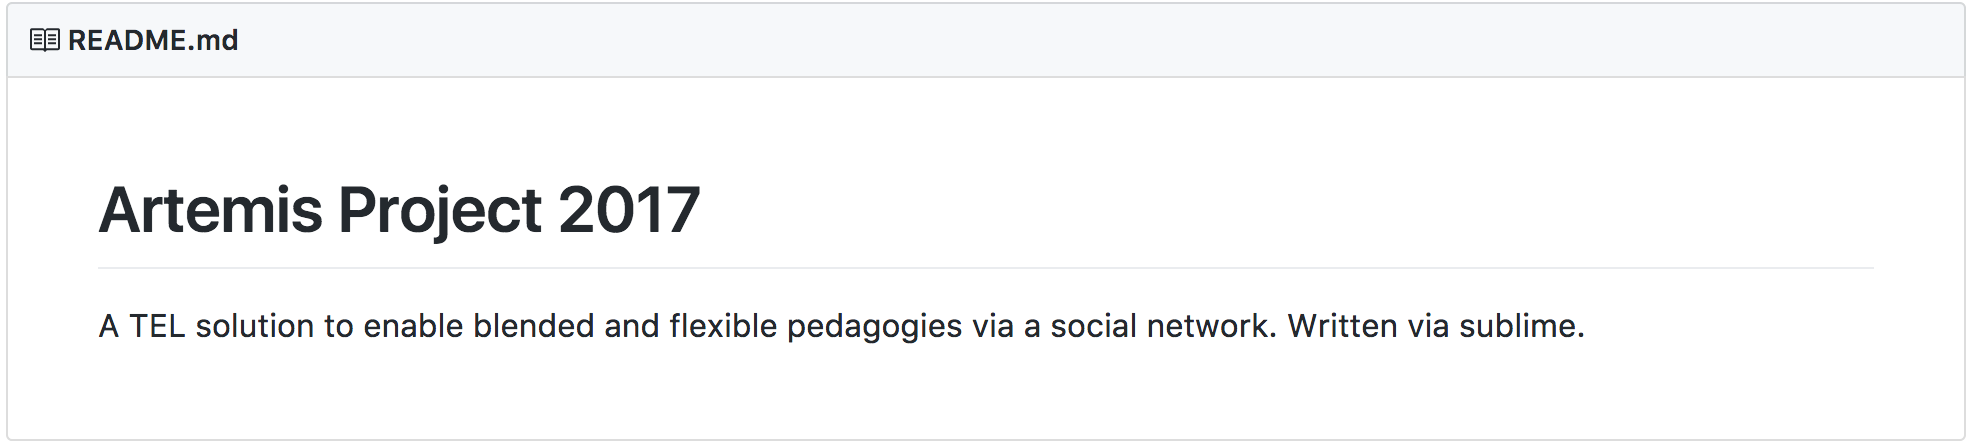
\includegraphics[scale=0.36]{chapters/chapter03/figures/readMe.png}}
                \caption{ReadMe Markdown File for Developers. Available at: \url{https://github.com/TaimurAhmed/summerProject2017}}
            \end{figure}
    \end{itemize}
    
    Furthermore UoB's offical favicons have been used (freely disseminated \cite{UniversityofBristola} and other default favicons were deprecated in favour of UoB's own logo \cite{UniversityofBristola} to further enhance user perception of a real organization. It is envisaged that if the tool is deployed in the future on UoB's in house servers this will further enhance this value as it will likely be disseminated via the organizations own web portal, giving users greater assurance within the relevant context (albeit Artemis is likely to have it's own domain name).


    \newpage    
    \item \textbf{"Highlight the expertise in your organization and in the content and services you provide."} \cite{Fogg2002a}:
    
   
   The Artemis Wiki as shown in the figure on \textbf{page \pageref{wiki}} has been used to highlight the technical aspects of Artemis e.g. the accessibility and security features behind Artemis via the content of the application. Furthermore the wiki is used to communicate the pedagogical rationale behind the project i.e. the design aspects and use cases. Effectively the wiki summarizes the technical and design features of the project for the benefit of users, so as to provide assurance in the expertise behind the project.
   
   The developer page which can also be accessed via Artemis can be used to highlight the expertise behind Artemis (ideally at the time of deployment an experienced team of developers will maintain the application and can reuse these links).
   
    \item \textbf{"Show that honest and trustworthy people stand behind your site"} \cite{Fogg2002a}:
    
    STPL recommends showing users that the people behind the web application are \textit{real} \cite{Fogg2002a}. This has been implemented in Artemis as follows:
    \begin{enumerate}
        \item Allowing for rich contextual data to be illustrated to the user when viewing other user's profiles i.e. users are able to determine that other profiles on the network either belong to fellow students or expert instructors.
        \item A separate page for biographical information of the developers as recommended by the STPL \cite{Fogg2002a} and illustrated on \textbf{page \pageref{developer}}.
        \item Making access to developer information and profiles available on all pages.
    \end{enumerate}
    
    \item \textbf{"Make it easy to contact you."} \cite{Fogg2002a}:
    
    This this can and has been done by simply adding developer contact details for bug reports, suggested improvements and feedback via the social networks to the UI i.e. the developers can be contacted via the click of a button in the nav bar of Artemis, which is accessible on every page of Artemis at all times. Furthermore detailed information is provided in the Wiki, ReadMe markdown, Bug and Error reporting page and developer's personal page to make it easy for users to contact the developer and learn more about the application.

    \item \textbf{"Design your site so it looks professional (or is appropriate for your purpose)"} \cite{Fogg2002a}:
    
    As recommended by STPL and implemented in this project , user acceptance testing was carried out to rigorously evaluate and subsequently refactor Artemis. User testers were intentionally encouraged to explore the application,  maliciously try to break it and undergo a series of Use Cases (See Appendix A1) unassisted. Whilst during the evaluation process the feedback was largely positive, a log of all issues was kept and all errors/user preferences were accounted for via code refactoring (Collated, identified and explained in a later chapter).

    \item \textbf{"Make your site easy to use"} \cite{Fogg2002a}:
    
    It was proposed during the focus group meeting with students that this can be done by seeking design inspiration from familiar social networks such as Facebook and Wikipedia, as users are likely to be familiar with the lay out and design of these sort of web applications\cite{Fogg2002a}. Furthermore the UI was evaluated and refactored as per user testing to enhance this aspect of user interaction and consideration  for assistive client side technologies such as screen readers or magnifiers was made with the use of ARIA (discussed in a later section of this chapter).
    
    \item \textbf{"Update your site's content often (at least show it's been reviewed recently)."} \cite{Fogg2002a}:
    
    Within the context of a Web 2.0 application that generates dynamically generated content contributed by the users, this should not necessarily be a problem. However after deployment the developer documentation that has been set up i.e. Wiki, Markdown file, Developer Page and Bug/Issue Report page, the relevant aspect of the project can be used to regularly update clients on recent releases and updates. This aspect is likely to be of more relevance after deployment and can only be anticipated preemptively. For the most part reasonable implementation is beyond the constraints of the project.
    
    \item \textbf{"Use restraint with any promotional content."} \cite{Fogg2002a}:
    
    As Artemis is not a commercial venture, this aspect of enhancing Web Credibility is easily addressed by using no promotional content.
    
    \item \textbf{"Avoid errors of all types, no matter how small they seem."} \cite{Fogg2002a}:
    
    The user evaluation testing was carried out without developer intervention and user testers were strongly encouraged to try and maliciously break and rigorously hack the program. This yielded valuable feedback used to refactor the code and will be discussed in a later chapter on evaluation and refactoring.
    
\end{enumerate}
\newpage


\section{Web Application Security}

With the transition of the world wide web from web-sites to web applications, i.e. the transition towards Web 2.0, a new host of security vulnerabilities moving away from traditional server side vulnerabilities towards new vectors such as vectors originating from client side have arisen \cite{Dayfdd2011}. Given the underlying importance of addressing common Web Application Security vulnerabilities \cite{Dayfdd2011} and it's negative impact on areas including but not limited to web credibility \cite{Fogg2002a,Fogg1999} that can affect the overall success and efficacy of the tool and even harm the users, this issue must be addressed for Artemis.

\subsection{OWASP}

An extensive review of web application security is desirable but beyond the reasonable constraints of this project. Therefore  utilising the \textit{Open Web Application Security Project (OWASP) Top 10} \cite{OWASP2017} for identifying common or important design vulnerabilities and mitigating them was  used during development, as a viable alternative achievable within the constraints of the project.

The Open Web Application Security Project is an online community  and  a respected  not-for-profit organisation which creates free to use articles, methodologies, documentation, tools, and technologies towards the benefit of web application security \cite{OWASP}. The organisation  annually releases research that identifies and underlines mitigation strategies for the \textit{"Ten Most Critical Web Application Security Risks"}\cite{OWASP2017} identified threat agents within the scope of qualitative benchmarks i.e. possible attack vectors, the prevalence and detectability of security vulnerabilities, the technical implications and the commercial/business implications.

The rationale behind these qualitative benchmarks to assist the quantification and ranking of security risks,  is illustrated as via the help of the following diagram which breaks a security vulnerability down into stages for classification and consideration:

% A single figure
\begin{figure}[H]
	\centering
	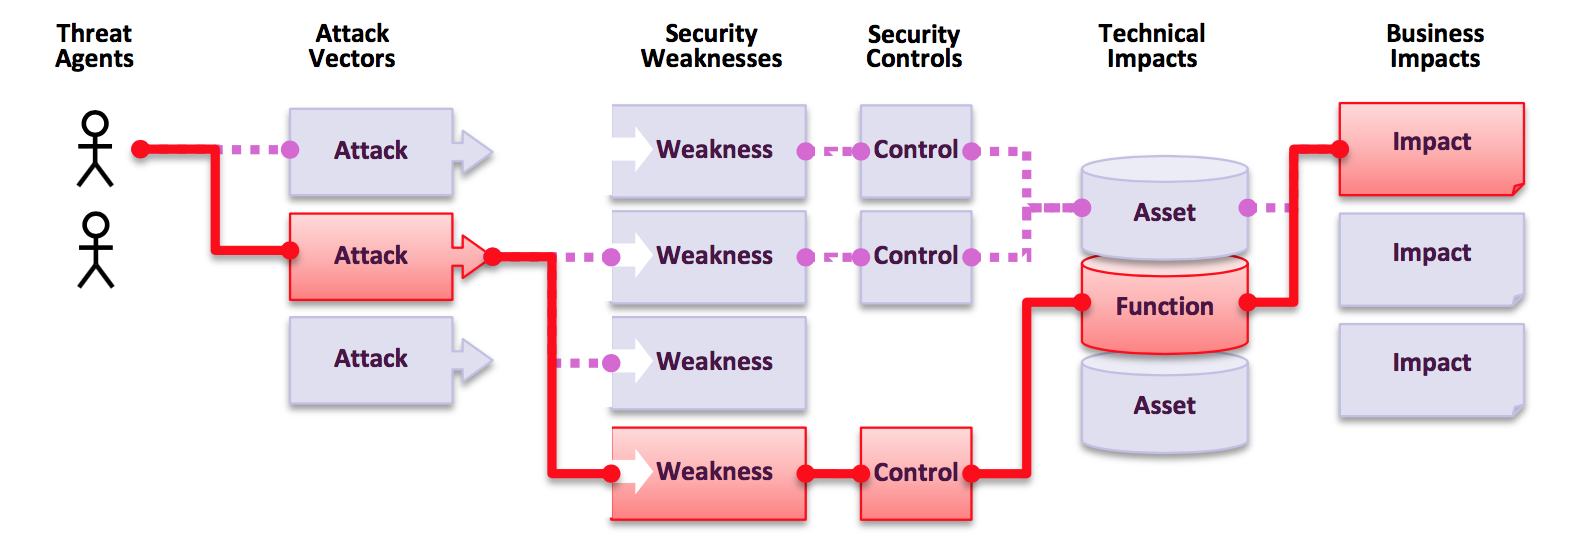
\includegraphics[scale=0.5]{figures/attack}
	\mycaption[Application Security - Consideration of Threat Agents]{Considerations of Threat Agents - . Figure reproduced from \cite{OWASP2017}.}
	\label{fig:Consideration of Threat Agents}
\end{figure}

The OWASP foundation reasons \cite{OWASP2017} that attackers or threat agents can exploit various modes of attack or \textit{attack vectors}, based on \textit{prevalence} and ease of \textit{detecting security weaknesses}/vulerabilities that can have a negative impact  within a generic technical or application specific commercial context \cite{OWASP2017}. Apart from application specific implications, the rest of these benchmarks can be classified based on the severity; which results in classification for the purpose of ranking the OWASP Top 10 vulnerabilities:

% A single figure
\begin{figure}[H]
	\centering
	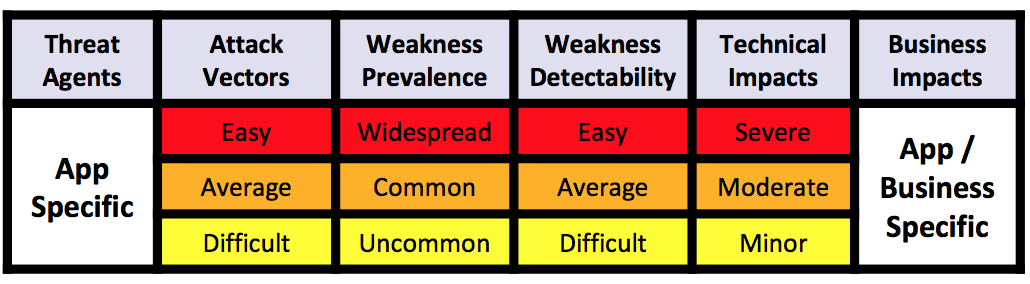
\includegraphics[scale=0.85]{figures/tabulation}
	\mycaption[OWASP Risk Rating Methodology]{OWASP Risk Rating Methodology - . Figure reproduced from \cite{OWASP2017}.}
	\label{fig:OWASP Risk Rating Methodology}
\end{figure}

Finally the risk rating methodology is used to compile an annual list of the most common, detectable and damaging security threats, along with mitigation strategies \cite{OWASP2017}. The proposed OWASP Top 10 for 2017, is effectively a mitigation strategy for this project that considers the likelihood and impact of security vulnerabilities. This seems to be a reasonable approach to security within the context of this project, as predicting attack vectors for every eventuality is not just futile but also undoubtedly unfeasible. Therefore within the context of the following attack vectors, Artemis has mitigated the risk as follows:

\begin{enumerate}
    \item \textbf{Injection}:
    
    \begin{figure}[H]
    	\centering
    	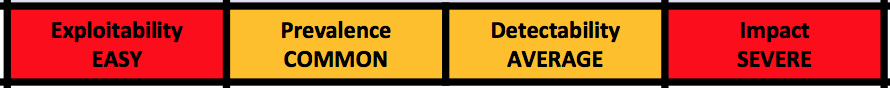
\includegraphics[scale=0.80]{figures/injection}
    	\mycaption[Injection Classification]{Injection Classification \cite{OWASP2017}.}
    	\label{injection}
    \end{figure}
    
    
    Injection vulnerabilities (particularly SQL injections) are the top vulnerability on the OWASP list \cite{OWASP2017}. As the figure below illustrates, it is an easily exploitable attack vector (as it is text based) and exploits interpretor syntax and can have a severe impact on an application e.g. MariaDB could be exploited by truncating all stored data or worse storing malicious data (The damage can be as severe as the hacker's imagination and ability).
    

    The most common cause of code injection i.e. SQL injection has been easily dealt with via the use of prepared statements to interact with the MariaDB in Artemis; otherwise known as a parameterised statement, a prepared statement is used to execute the same statement repeatedly with high efficiency and prevent SQL injection as per the PHP API\cite{PHP}. The use of prepared statements eliminates the possibility of SQL injection and avoid the pitfalls of relying on \textit{Escaping Strategy} (albiet as an extra layer of security Artemis does use PHP's native MySQLi escape methods, despite not actually being necessary in lieu of prepared statements), which can be notoriously hard to implement perfectly.
    
    To completely mitigate this attack vector within the context of Artemis, all user input is  sanitized via PHP's native \textit{strip\_tags} function. As per the PHP manual this sanitizes all PHP and HTML code into ordinary strings. Effectively the relevant interpreters have been insulated from user injected code and this risk has been almost eliminated in Artemis.
    
    In summary code injection has been prevented as follows:
    \begin{enumerate}
        \item Sanitizing User Input.
        \item Escaping User Input.
        \item Parameterised/Prepared Statements for storing sanitised and escaped user input into MariaDB.
    \end{enumerate}
    
    \begin{figure}[h]
    	\centering
    	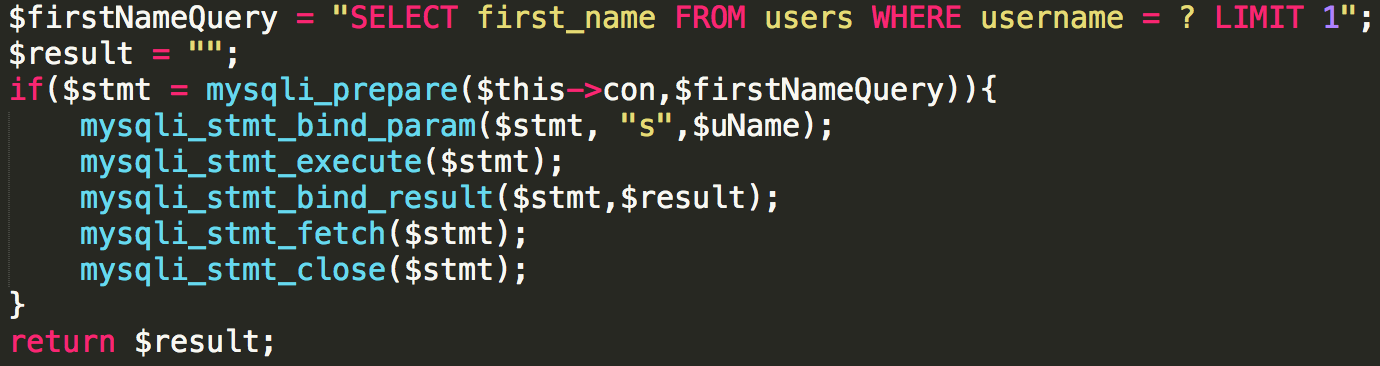
\includegraphics[scale=0.61,right]{chapters/chapter03/figures/preparedStmt.png}
    	\mycaption[Example Example Prepared Statementt]{Example Prepared Statement.}
    	\label{Example Prepared Statement}
    \end{figure}
    

    \item \textbf{Broken Authentication and Session Management}:
    
    Authentication and/or session management functionality are often implemented incorrectly \cite{OWASP2017}. Effectively this could allow malicious attackers to compromise passwords, keys, or session tokens, and other flaws via assuming a victim's identity on the social network \cite{OWASP2017}.
    
    OWASP PHP Security project finds that the PHP's default session facility is safe and generates a session id that is sufficiently random \cite{OWASPa}. However the project does recommend steps to prevent common attack vectors within this category such as session hijacking. These have been addressed as follows:
    
    \newpage
    
    \begin{enumerate}
        \item \textbf{Session Hijacking}: 
        \begin{enumerate}
            \item Session Fixation\cite{OWASPa} and Rolling Session ID's: After a successful user login and with each page visit the session id has been regenerated using the PHP function \textit{session\_regenerate\_id}. Effectively each page visit invalidates the last session id reducing the risk of compromise due to a hijacked session.
            \item Invalidate Session ID: Incorrect session ID's are invalidated and users are forcefully redirected to the application log in page, regardless of which page they are on via the use of header.php.
            \item Session Expiration: Sessions are expired after 30 seconds of inactivity as per OWASP reccomendations, using the PHP function \textit{session\_set\_cookie\_params}
        \end{enumerate}
        \item \textbf{Cookie Management}:
        OWASP \cite{OWASPa} recommends standard good security practices such as not serializing cookie data (due to an increased scope of security concerns) or storing sensitive data in a cookie (which can easily be accessed by a hacker or even the user themselves).  These have been incorporated in Artemis's design.
        \begin{enumerate}
            \item Cookie Parameters: The \textit{cookie\_params} function has been used to secure the cookie settings for artemis. This involves:
                \begin{itemize}
                    \item Setting a cookie lifetime (an arbitrary 30 seconds).
                    \item Path on the domain where the cookie will work; Currently set to work on the entire domain but will need to be reconfigured on deployment.
                    \item Cookie domain, currently local host but will need to be reconfigured as reasonable at the time of deployment.
                    \item Secure connection transport protocol; See below for details on SSL.
                    \item Enabling HTTP only session cookies;See below for details.
                \end{itemize}
                Clearly not all of cooke settings security features can not be factored in during development by default as some of them rely on the existence of an actual domain name i.e.SSL,HTTP/HTTPS, domains and path. A self signed certificate in these instances is at best a half measure and would ultimately need to be replaced once an actual domain is secured. Therefore clear and explicit disclosure has been made in developer documents regarding re-factoring at the time of deployment and within the source code itself; Toggling these security features is as simple as changing a boolean value, which is deemed not unnecessarily onerous as long as it is clearly disclosed.
        \end{enumerate}
    \end{enumerate}

    \item \textbf{Cross Site Scripting (XSS)}:
    
    XSS vulnerabilities include the inclusion of untrusted data in a new web page without proper validation or escaping; particularly problematic with browser API's that create JS. Depending on the application use case XSS mitigation can take many forms. Given that HTML and PHP tags as user input are not necessary in Artemis, this risk has been completely mitigated by using the sanitisation strategy mentioned during the mitigation of code injection. The user unput sanitisation strategy which relies on stripping HTML, PHP tags and   special HTML entities conversion to ordinary strings has the added advantage of completely mitigating XSS.
    
    \textbf{Security Extension: Self XSS}:
    While OWASP doesn't specifically identify guarding against Self XSS as a major security; An inspection of the  the client side code for FaceBook and Google Hangouts reveals that mainstream social networks warn users against self XSS attacks i.e. a social engineering attack vector where malicious hackers convince users to execute code in a browser console so as to compromise their own web security \cite{FaceBook}. An example of Facebook warning it's users against self xss is illustrated below:
    
    \begin{figure}[h]
    	\centering
    	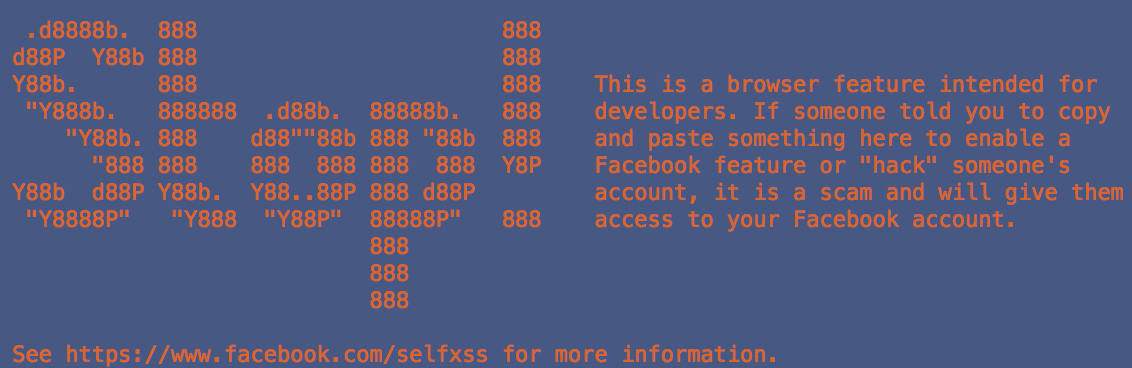
\includegraphics[scale=0.75,right]{chapters/chapter03/figures/faceBook.png}
    	\mycaption[FaceBook Self XSS Warning]{FaceBook Self XSS warning in browser console.}
    	\label{faceBookSelfXSS}
    \end{figure}
    
    As the figure above illustrates this a simple console message, meant to grab the attention of the client; should they access developer tools in their browser. Therefore it was adopted in Artemis's design which warn's its own users against Self XSS (as illustrated below). It is reasoned that if main stream social networks have adopted this practice, it is not unreasonable to do the same. Note that the console message below has been designed in a manner to catch the users attention, before they try to attempt anything.
    
    \begin{figure}[h]
    	\centering
    	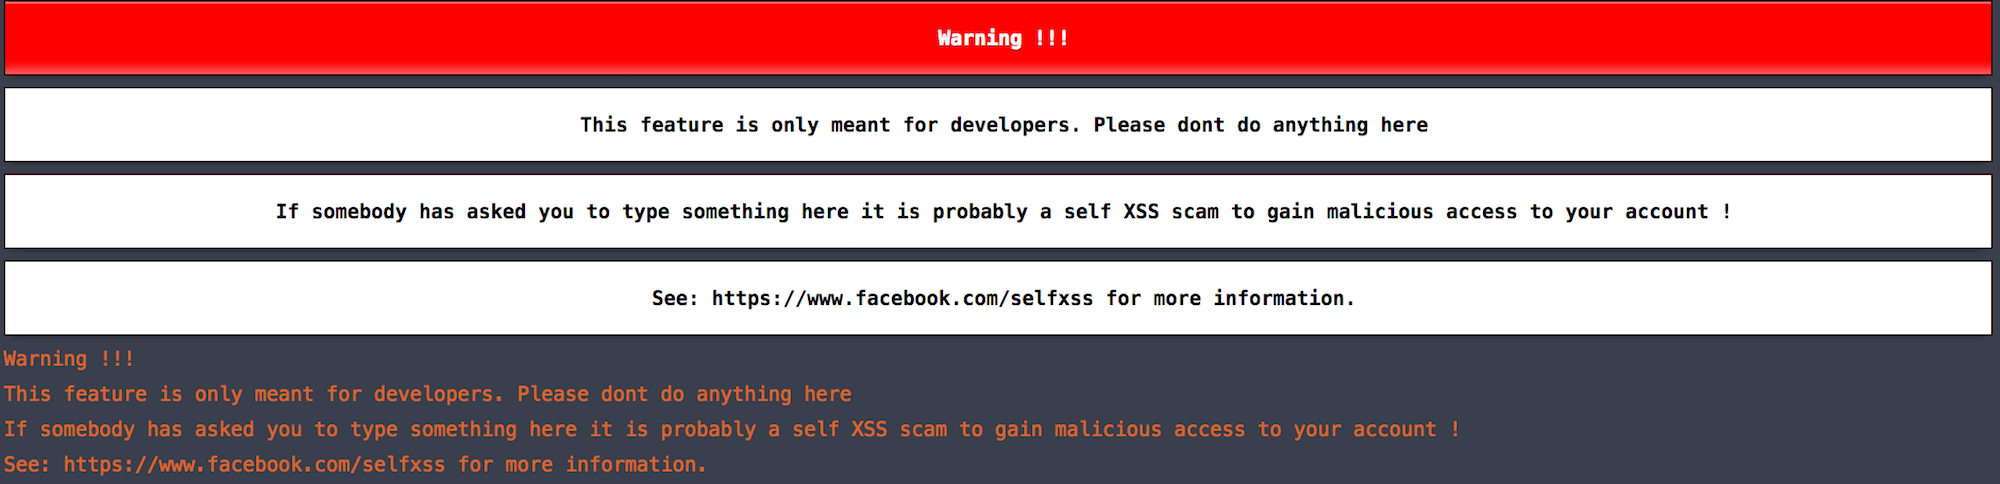
\includegraphics[scale=0.44,right]{chapters/chapter03/figures/ArtemisXSS.png}
    	\mycaption[Artemis Self XSS Warning]{Artemis Self XSS warning in browser console.}
    	\label{ArtemisSelfXSS}
    \end{figure}   
    
    
    
    \newpage
    
    \item \textbf{Broken Access Control}:
    
    A White Listing or Black Listing strategy was considered for the purposes of Artemis, but was deemed onerous for implementing within the context of a dynamically generated application of it's design. Artemis makes use of server side and database logic to serve various access control relevant features such as personal messages, comments, newsfeed, bio etc. Therefore it is realistically not possible (assuming no human error) to view information that a person does not have access to, if the server side DB logic does not concur. E.g. If a person tries to access the newsfeed of a person they are not friends with via direct object reference, it is not possible as they will be redirected to a 'limited' view of the relevant person's profile.
    
    Admittedly this does the raise some ethical concerns such as the need to block malicious users in the case of cyber bullying. However this is not relevant to Web Security and will be discussed in the concluding chapter of this report.
    
    \item \textbf{Security Misconfiguration}:
    
    As per OWASP \cite{OWASPa} PHP is by default an insecure language for deployment. The reason for this is that PHP needs to be reconfigured to switch from development mode to settings more suitable for deployment e.g. by default DB errors will lead to a PHP application leaking sensitive server and directory information which a hacker can use to probe an application and discover vulnerabilities. The file responsible for configuring php is known as \texxit{php.ini} or the \texxit{configuration file}\cite{PHPa}.
    
    The configuration file allows for useful settings to be turned on such as detailed error messages during development. However what is an asset during development is usually a major liability during production or deployment. Therefore a php.ini file has been shared in the project; solely for the purpose of deployment as opposed to development.
    
    The configuration file has been broken up as follows and is explained accordingly \cite{OWASPa}:
    \begin{itemize}
        \item \textbf{PHP Error Handling}\cite{OWASPb}: OWASP's PHP project recommends the following settings  illustrated below. The underlying rationale here is to turn off features such as compiler warnings that may reveal sensitive information about the source code of the program. Whilst these settings are helpful during development they are not suitable from a security perspective during production.
            \begin{figure}[H]
            	\centering
            	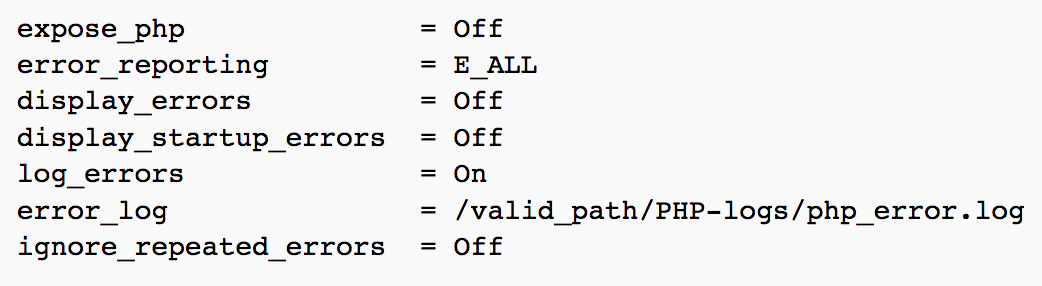
\includegraphics[scale=0.44,center]{chapters/chapter03/figures/errorPHP.png}
            	\mycaption[PHP Error Handling Configuration]{PHP Error Handling Configuration}
            	\label{PHPError}
            \end{figure}   

        \item \textbf{PHP General Settings}\cite{OWASPb}: URL routing and default directory setup is usually vulnerable in PHP. The following settings are good practice and prevent scenarios such as easy escalation of local file inclusion to remote file inclusion and explicitly setting the document root folder.
        
            \begin{figure}[H]
            	\centering
            	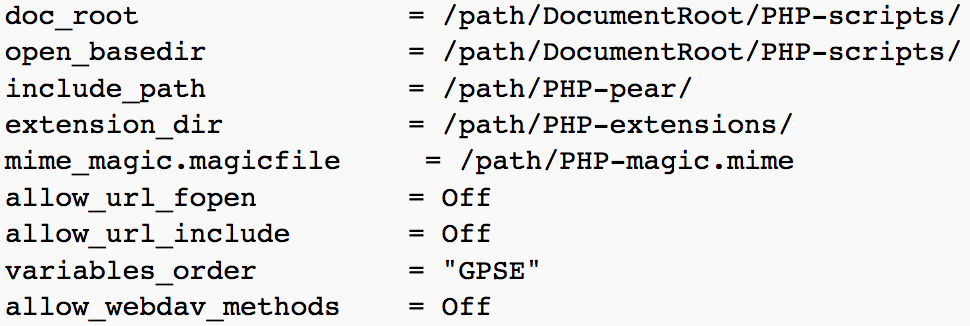
\includegraphics[scale=0.44,center]{chapters/chapter03/figures/generalPHP.png}
            	\mycaption[PHP General Configuration]{PHP General Configuration}
            	\label{PHPGeneral}
            \end{figure}   
        
    
        \item \textbf{PHP Executable Handling\cite{OWASPb}: OWASP} \cite{OWASPb} explicitly identifies the following as extrenely insecure function in PHP which need to be turned off unless explicitly necessary, as they can be exploited by hackers. As Artemis does not use them they are deemed unnecessary:
            
            \begin{figure}[H]
            	\centering
            	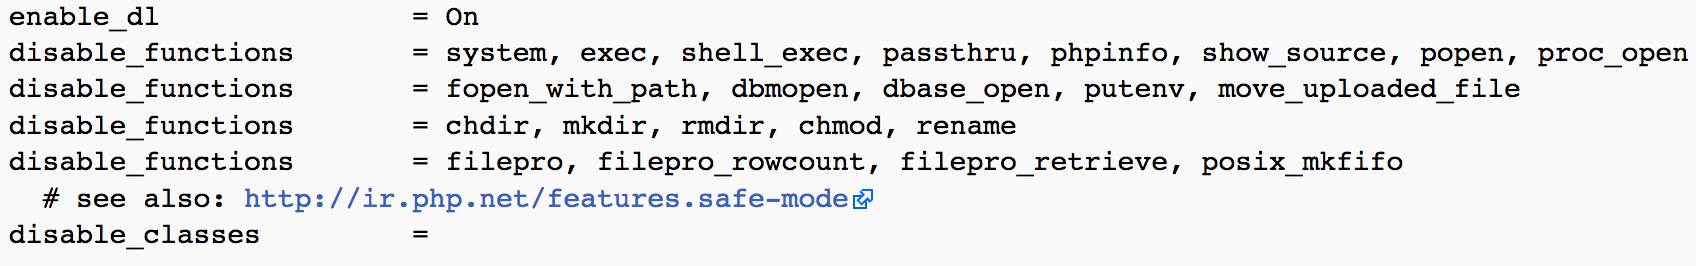
\includegraphics[scale=0.44,center]{chapters/chapter03/figures/execPHP.png}
            	\mycaption[PHP Executable Handling Configuration]{PHP Executable Handling Configuration}
            	\label{PHPExec}
            \end{figure}

        \item \textbf{PHP Session Handling}\cite{OWASPb}:

            \begin{figure}[H]
            	\centering
            	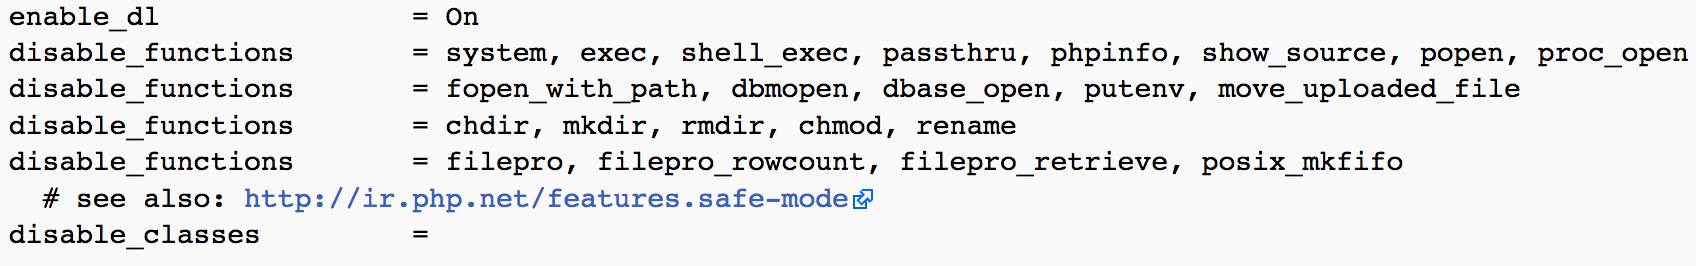
\includegraphics[scale=0.44,center]{chapters/chapter03/figures/execPHP.png}
            	\mycaption[PHP Session Handling Configuration]{PHP Session Handling Configuration}
            	\label{PHPSess}
            \end{figure}       

    \end{itemize}
    
    
    
    \item \textbf{Sensitive Data Exposure}:
    
    Particularly relevant to web applications such as this project which collect social data, APIs do not properly protect sensitive data, which attacker may misuse. OWASP recommends modern encryption strategies to mitigate the risk of security breaches, anticipated or otherwise, e.g. using strong purpose built algorithms and simply dropping data from databases that regularly, that is not useful for commercial/app specific purposes \cite{OWASP2017}.
    
    \item \textbf{Insufficient Attack Protection}:
    
    This refers to app vulnerabilities such as APIs which lack the basic ability to detect, prevent, and respond to both manual and automated attacks \cite{OWASP2017}. It bears noting that this area covers proactive and reactive mitigation strategies well beyond the scope of the project, despite considerations that may be given to blocking automated and manual malicious attacks during the course of development.
    
    \item \textbf{Cross Site Request Forgery (CSRF)}:
    
    A CSRF attack forces a logged-on victim's browser to send a forged HTTP request, including the victim’s session cookie and any other automatically included authentication information, to a vulnerable web application \cite{OWASP2017}. Already introduced mitigation strategies for other aspects such as cookie management, session hijacking, injection and sanitisation reduce the possibility of this vector as it usually relies on social engineering and malicious code.
    
    However as CSRF attack usually misuses a web application to create undesired affects, special emphasis has been placed on particularly sensitive data such as account settings which involve changing the password. In this instance the \textit{Google Recaptcha V2 API} was utilised to add an extra layer of security to prevent CSRF. Furthermore the optional IP tracking argument has been used to deploy the Recaptcha to track malicious activities. The implementation is illustrated as follows:
  
    \begin{figure}[h]
    	\centering
    	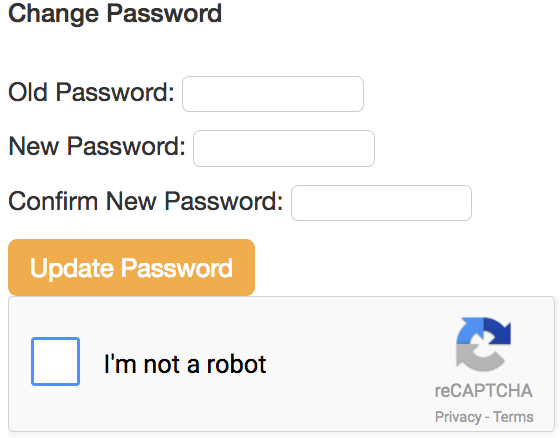
\includegraphics[scale=0.44,center]{chapters/chapter03/figures/captchaGoogle.png}
    	\mycaption[Google ReCaptcha]{Google ReCaptcha. Request on Artemis Accounts Settings Page.}
    	\label{googleRecaptcha}
    \end{figure}  
    
    \newpage
    
    \begin{figure}[h]
    	\centering
    	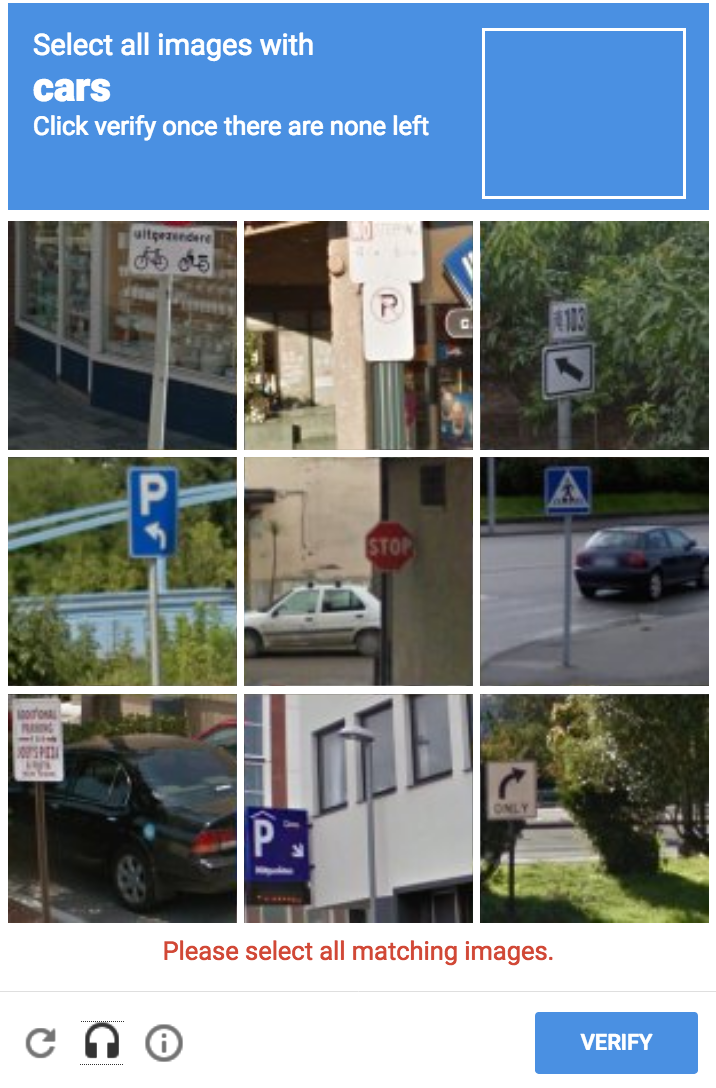
\includegraphics[scale=0.44,center]{chapters/chapter03/figures/verifyGoogle.png}
        \mycaption[Google ReCaptcha]{Google ReCaptcha. Test.}
        \label{ArtemisSelfXSS}
    \end{figure}  
    

    
    
    
    \item \textbf{Using Components with Known Vulnerabilities}:
    
    Components, such as libraries, frameworks, and other software modules, run with the same privileges as the application and if a vulnerable component is exploited,  an attack can facilitate  a plethora of malicious activities \cite{OWASP2017}.
    
    Most mitigation strategies in this area are usually reactive (beyond researching components before using them), thus deemed outside of the constraints of this report.
    
    \item \textbf{Underprotected API's}:
    
    "Modern applications often involve rich client applications and APIs, such as JavaScript in the browser and mobile apps, that connect to an API of some kind (SOAP/XML, REST/JSON, RPC, GWT, etc.). These APIs are often unprotected and contain numerous vulnerabilities" \cite{OWASP2017}.
    
    This is a relatively new area of vulnerability being studied for the purpose of mitigation strategies by OWASP \cite{OWASP2017}; generally beyond the reasonable constraints of this project. A proposed mitigation strategy available here, is to perhaps consider expert advise from security experts and practitioners of relevant client applications.
    
\end{enumerate}




\section{Accessibility}

Making a tool user accessible is an important consideration when deploying a TEL solution, within the context of UoB students as per preliminary meetings with the UoB TEL team. Furthermore user accessibility enhances both the persuasiveness of the TEL solution and it's web credibility. However it is recognised that accessibility issues can cover a wide range of impairments within the broad blanket categories such as audio, visual and mobility impairments \cite{Mills2015}. An extensive accessibility review for this project, is beyond it's reasonable constraints as mitigation for every possible impairment is impossible to implement, and is usually reactive in nature as per the UoB TEL team.

It is proposed that by following best practice on at least visual impairment (likely the most important of the three within the context of this project) as recommended by the MDN's (Mozilla Developers Network) guidelines \cite{Mills2015,Mills2016} on accessibility and W3C's (World Wide Web Consortium) Web Accessibility Initiative (WAI) for developers \cite{W3C}, a satisfactory level of accessibility can be embedded in the design of the tool.

\subsection{Accessible HTML, CSS and JavaScript}

HTML, CSS and JavaScript are basic building blocks in most web applications such as the proposed social network and by following specific best practice at the time of development to enhance accessible device interaction, the need for using tools such as WAI-ARIA can be reduced \cite{W3C,OWASP,Mills2015,Mills2016}. As opposed to CSS and JavaScript, HTML is cited as having the greatest implications (negative and positive)  within the context of interaction with relevant accessibly devices e.g. screen readers \cite{Mills,Mills2017} and ultimately an impact on user accessibility.  It is highlighted that the nuances of enhancing accessibility are different for all of the aforementioned technologies; however they are condensed in the interest of brevity into overlapping points of best practice as follows:


\begin{enumerate}
    \item \textbf{Semantically Sensible Code}:
    
    This refers to the use of the correct semantic language elements for the correct purpose e.g. using breaks, paragraphs and specific HTML tags for intended purposes only \cite{Mills,Mills2017} to create a semantically sensible layout of data, so that screen readers which are developed with certain expectations/assumptions can operate correctly.
    
    Within the context of HTML this refers to using semantic HTML otherwise referred to as POSH (plain old semantic html) HTML \cite{Mills2017} and for CSS and JavaScript (JS) using semantically sensible code \cite{Mills}. The rationale for using semantically similar and plain code is that it is more likely to conform to client-device expectations and result in a smoother user interaction experience via accessibility devices such as screen readers \cite{Mills2017,Mills}.
    
    \item \textbf{Unobtrusive and Flexible Code}:
    
    Client side devices such as screen readers effectively take control of the code in a web application, which for the sake of accessibility as well as technical flexibility should be accepted during development e.g. users may override CSS to use custom style sheets to read content more easily \cite{Mills}. Beyond merely accepting the possibility of overriding control, CSS and JS in particular should be developed to make this easier for screen readers and accessibility devices \cite{Mills,Mills2017,Sukardi2016} i.e. writing flexible code that is unobtrusive towards user devices e.g. Developing client-side form validation, which alerts users to problems with their form entries quickly,as opposed to server-side form validation which would take longer and cause problems or confusion from the perspective of a visually impaired user using a screen reader. 
    
    Assuming the usage of POSH HTML, this requirement extends to writing more flexible and unobtrusive CSS and JS. As such it would be impractical to envision and identify every possible use case, however it suffices to say that writing flexible and unobtrusive code is not always possible given the complexity of modern UI's that require unsemantic HTML5 features and dynamic content generating JS, indicative that alternative tools will be necessary as well \cite{Mills,Sukardi2016}, discussed in the next section.


    \item \textbf{Colour Contrast}:
    
    
    MDN guidelines recommend accommodating  colour blind accessibility via the use of colour contrast checkers during web development \cite{Mills}. This would can allow for iterative testing during the development process, to assess whether the site is readable from the perspective of a colour blind person and more than merely aesthetically pleasing CSS. It is also recommended to use non-colour alternatives  to aid document semantics, along with colour based semantic aids \cite{Mills} e.g. altering the fonts along with font colour to highlight text, effectively making the highlighted text visible to colour blind users. By using non-visual cues, people impaired by colour blindness are more easily able to detect patterns and text.
    
\end{enumerate}

\subsection{WAI-ARIA (Web Accessibility Initiative - Accessible Rich Internet Applications)}

Semantically well formed HTML, CSS and JS is recommended as a first port of call for making UI's accessible \cite{Sukardi2016}. However as discussed earlier, given the complexity of a social network's UI which is almost certainly going to use  dynamic JS updated content, if not unsemantic HTML5 features an alternative tool is necessary \cite{Sukardi2016}.


In such instances WAI-ARIA  \cite{W3C,February2016a,Sukardi2016} seem to be the viable alternative for this project. WAI is a specification written by the W3C \cite{W3C,Sukardi2016} which adds additional semantic attributes to a web application's HTML. ARIA is a technology that can help  by adding in further semantics that browsers and assistive technologies can recognize and use, benefiting the user experience of accessibility challenged clients \cite{W3C,Sukardi2016}. 

ARIA technology is supported by W3C via the WAI \cite{W3C,February2016a}, has good global browser support \cite{Sukardi2016} and is supported by most major screen reader used in the area \cite{Sukardi2016}. ARIA has many features and resultant use cases, some of which might not be relevant or feasible for this project \cite{February2016a}.Within the context of this specific project WAI-ARIA's many tools can be used for the following :

\begin{enumerate}
    \item Semantic Enhancement: WAI-ARIA can enhance the semantic attributes of HTML for this project. Alternatively, it can be used to replicate HTML semantics where none are possible to implement via HTML itself.
    \item Dynamic content updates: The use of dynamically updated content via JS is unavoidable for this project, which unfortunately screen readers tend to have difficulty with \cite{Sukardi2016,Mills}. ARIA utilises technology that can inform screen readers of content updates to the screen and effectively any new content generated in a social  network \cite{Sukardi2016}.
    \item Assisting Non-Semantic Complex UI's and Control: UI's or menus that utilise nested HTML div tags, along with JS and CSS can benefit from advanced control features, however interpreting them from the perspective of a screen reader device can be very difficult. ARIA provides functions and tools, capable of providing clues to a screen reader as to how to go about navigating a complex UI.
\end{enumerate}

Before concluding this chapter it must be reiterated that accessibility is a desirable feature for this project. However an extensive  review to make the web application accessible for all eventualities is deemed unfeasible in light of the project constraints. Therefore the whilst certain accessibility mitigation strategies such as semantic,flexible and unobtrusive programming for HTML,CSS and JS will be incorporated into design, evaluation via screen readers and embedding ARIA enhanced semantics where necessary will  implemented as an optional deliverable/extension, if the project constraints allow it.


